\section{Conducto-convection à l'interface d'un\\solide et d'un fluide}

    \subsection{Transfert conducto-convectif : loi de Newton empirique}

        \subsubsection{Flux surfacique conducto-convectif}

            On fait l'hypothèse que le fluide est brassé par convection : $T_{f}$ est uniforme, voir la Figure~\ref{fig:transfert_conducto_convectif_fluide_brasse}.

            \begin{figure}
                \centering
                \tikzsetnextfilename{transfert_conducto_convectif_fluide_brasse}
                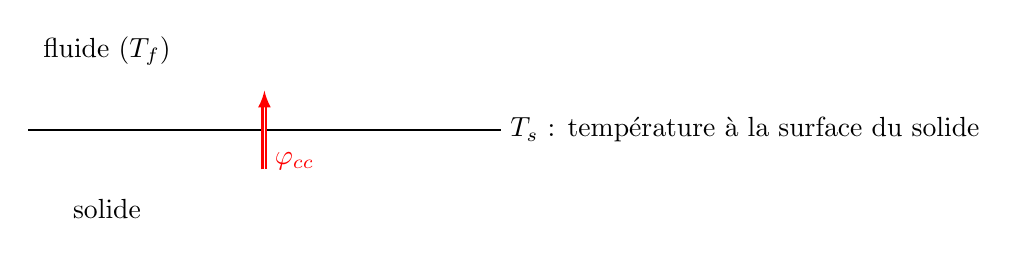
\begin{tikzpicture}[scale=1]  
                    % \helpgrid{3}{3}
                    \draw (-3,0)--(3,0) node [right] {$T_s$ : température à la surface du solide};
                    \node at (-2,-1) {solide};
                    \node at (-2,1) {fluide $(T_f)$};
                    \draw[->,double,-latex,thick,red,text=red] (0,-0.5)--++(0,1) node [right,pos=0.1] {$\varphi_{\text{cc}}$};
                \end{tikzpicture}
                \caption{Flux surfacique conducto-convectif.}    
                \label{fig:transfert_conducto_convectif_fluide_brasse}
            \end{figure}

            Le flux surfacique conducto-convectif est proportionnel à $T_s-T_f$. La loi de Newton s'écrit dans ce cas
            \begin{equation*}
                \boxed{
                    \varphi_{\text{cc}}=h\left(T_s-T_f\right).
                }
            \end{equation*}
            L'unité de $\varphi_{\text{cc}}$ est \si[]{\watt\per\metre\square} et est orienté du solide vers le fluide. Le facteur $h$ est le coefficient de transfert conducto-convectif d'unité \si[]{\watt\per\metre\square\per\kelvin}.
            Ainsi,
            \begin{equation*}
                \boxed{
                    P_{s\to f}=\varphi_{\text{cc}}\times S=hS\left(T_s-T_f\right).
                }
            \end{equation*}

            \paragraph{Ordre de grandeur.} Pour le gaz, $h\sim 5$ à 30 \si[]{\watt\per\metre\square\per\kelvin}, pour le liquide, $h\sim 400$ à 10000 \si[]{\watt\per\metre\square\per\kelvin}, les deux pour la convection naturelle. Si le convection est forcée, on a un rapport 
            \begin{equation*}
                \frac{h_{\text{forcée}}}{h_{\text{naturelle}}}\sim 10\text{ à }50.
            \end{equation*}

        \subsubsection{Interprétation}

            Lors d'un écoulement fluide, il y a deux zones : une proche du sol, dite \og couche limite\fg. L'autre est lointaine, c'est l'écoulement extérieur. Alors
            \begin{equation*}
                \varphi_{\text{cc}}=j_{\text{th},C.L}=-\lambda_f\left(\frac{\partial T}{\partial x}\right)_{\text{fluide}}\approx-\lambda_f\frac{T_f-T_s}{\delta},
            \end{equation*}
            où $\delta\ll$ taille macroscopique de l'écoulement (taille de la couche limite). Dans la couche limite, le transfert thermique (pas dû à la convection mais à la conduction thermique dans la couche limite) a lieu perpendiculairement aux mouvement du fluide. Donc 
            \begin{equation*}
                \varphi_{\text{cc}}\approx\frac{\lambda_f}{\delta}\left(T_s-T_f\right),
            \end{equation*}
            d'où
            \begin{equation*}
                \boxed{
                    h=\frac{\lambda_f}{\delta}.
                }
            \end{equation*}

            Comme $h\propto\lambda_f$, on a 
            \begin{equation*}
                \boxed{
                    h_{\text{liquide}}\gg h_{\text{gaz}}.
                }
            \end{equation*}
            Comme $h\propto1/\delta$, et $\delta$ diminue si le brassage augmente, on a 
            \begin{equation*}
                \boxed{
                    h_{\text{forcée}}\gg h_{\text{naturelle}}.
                }
            \end{equation*}

    \subsection{Application : ailette de refroidissement}

        On considère le système présent à la Figure~\ref{fig:application_ailette_refroidissement_conducto_convection}. On fait l'hypothèse que l'on est en régime stationnaire, que le problème est unidimensionnel ($T$ ne dépend que de $x$), et que la longueur de l'ailette est \og infinie\fg.

        \begin{figure}
            \centering
            \tikzsetnextfilename{application_ailette_refroidissement_conducto_convection}
            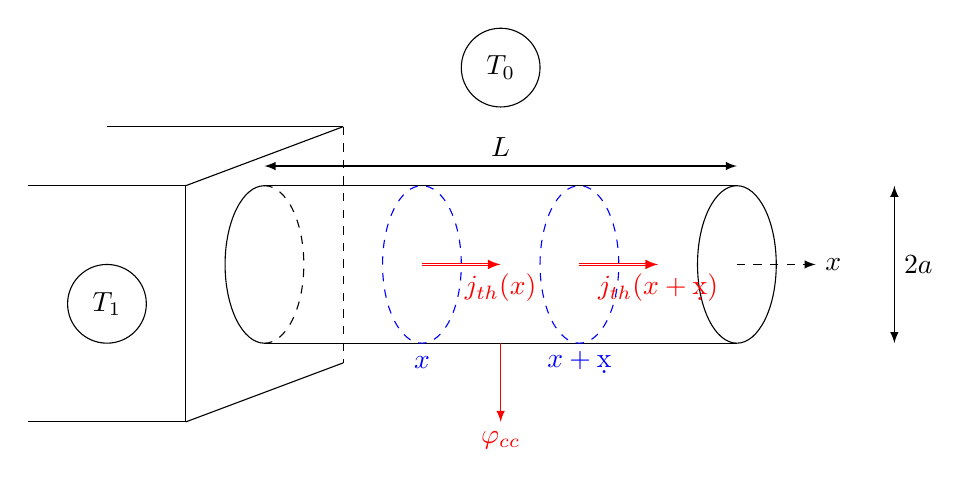
\begin{tikzpicture}[scale=1]  
                % \helpgrid{3}{3}
                
                \draw (-3,1)--(3,1);
                \draw (-3,-1)--(3,-1);
                \draw[latex-latex] (-3,1.25)--(3,1.25) node [above, midway] {$L$};
                \draw[latex-latex] (5,-1)--(5,1) node [right, midway] {$2a$};
                \draw (-3,1) arc[start angle=90, end angle=270, x radius=0.5, y radius=1];
                \draw [dashed] (-3,1) arc[start angle=90, end angle=-90, x radius=0.5, y radius=1];
                \draw [smooth] (3,0) ellipse (0.5 and 1);
                \draw[dashed, -latex] (3,0)--++(1,0) node [right] {$x$};

                \draw [dashed, blue] (-1,0) ellipse (0.5 and 1);
                \draw [dashed, blue] (1,0) ellipse (0.5 and 1);
                \node [text=blue] at (-1,-1.25) {$x$};
                \node [text=blue] at (1,-1.25) {$x+\d x$};

                \draw (0,2.5) circle (0.5) node {$T_0$};
                \draw (-5,-0.5) circle (0.5) node {$T_1$};
                
                \coordinate (A) at (-5,1.75);
                \coordinate (B) at (-2,1.75);
                \draw (A)--(B);
                \coordinate (C) at (-6,1);
                \coordinate (D) at (-4,1);
                \draw (C)--(D);
                \draw (B)--(D);
                \coordinate (E) at (-6,-2);
                \coordinate (F) at (-4,-2);
                \draw (E)--(F);
                \draw (D)--(F);
                \coordinate (G) at (-2,-1.25);
                \draw[dashed] (B)--(G);
                \draw (F)--(G);

                \draw[double,-latex,red,text=red] (-1,0)--++(1,0) node [below] {$j_{\text{th}}(x)$};
                \draw[double,-latex,red,text=red] (1,0)--++(1,0) node [below] {$j_{\text{th}}(x+\d x)$};
                \draw[-latex,red,text=red] (0,-1)--++(0,-1) node [below] {$\varphi_{\text{cc}}$};
            \end{tikzpicture}
            \caption{Application du flux conducto-convectif : ailette de refroidissement.}    
            \label{fig:application_ailette_refroidissement_conducto_convection}
        \end{figure}

        \subsubsection{Profil $T(x)$}

            On ne peut pas utiliser l'équation de la chaleur, il faut passer par un bilan d'énergie local sur $[x,x+\d x]$. En régime permanent, on a 
            \begin{align*}
                \frac{\d\left(\delta U\right)}{\d t}
                &=
                0,\\
                &=
                P_{\text{th}}^{\text{ext}},\\
                &=
                j_{\text{th}}(x)\pi a^{2}-j_{\text{th}}(x+\d x)\pi a^{2}-h(T(x)-T_0)2\pi a\d x.
            \end{align*}
            Ainsi, on obtient
            \begin{equation*}
                \pi a^{2}\frac{\partial j_{\text{th}}}{\partial x}\d x+h(T(x)-T_0)=0.
            \end{equation*}
            On pose $\theta(x)=T(x)-T_0$, et $\delta\coloneqq\sqrt{\dfrac{a\lambda}{2h}}$, et on obtient 
            \begin{equation*}
                \theta(x)=\alpha\e^{-x/\delta}+\beta\e^{x/\delta}.
            \end{equation*}
            On a $\beta =0$ car $\theta$ est fini en $+\infty$, et $\theta(0)=T_1-T_0=\alpha$. Finalement,
            \begin{equation*}
                \boxed{
                    T(x)=T_0+(T_1-T_0)\e^{-x/\delta}.
                }
            \end{equation*}

            Notons que si l'ailette est \og finie\fg, c'est-à-dire $L\sim\delta$, la condition au limite est alors donnée par la \textbf{continuité du flux en $x=L$}, c'est-à-dire 
            \begin{equation*}
                \varphi_{\text{cc}}(L)=j_{\text{th}}(L),
            \end{equation*}
            soit
            \begin{equation*}
                \boxed{
                    h(T(L)-T_0)=-\lambda\left(\frac{\partial T}{\partial x}\right)_{L}.
                }
            \end{equation*}

        \subsubsection{Efficacité}

            Sans l'ailette, la puissance thermique est $P_{\text{sans}}=h(T_1-T_0)S$, et la puissance avec l'ailette est $P_{\text{avec}}=-\lambda\left(\frac{\partial T}{\partial x}\right)_{0}S$. Ainsi, l'efficacité est 
            \begin{align*}
                \eta\coloneqq
                &=
                \frac{P_{\text{avec}}}{P_{\text{sans}}},\\
                &=
                \frac{\lambda\left(\frac{T_1-T_0}{\delta}\right)S}{h(T_1-T_0)S},\\
                &=
                \frac{\lambda}{\delta h}=\sqrt{\frac{2\lambda}{ah}}.
            \end{align*}

            On a $\eta\sim 30$ pour $\lambda\approx100$\si[]{\watt\per\metre\per\kelvin}, $h\approx10$\si[]{\watt\per\metre\square} et $a\approx2.10^{-2}$\si[]{\metre}.

    \subsection{Nombre de Biot : conduction versus conducto-convection}
        \subsubsection{Validité de l'hypothèse de l'ailette}
            L'hypothèse de l'ailette est que la température est uniforme sur une section. Si $T$ n'est pas uniforme sur une section, on décompose le flux $\vec{j}_{\text{th}}=\vec{j}_{\text{th},\perp}+\vec{j}_{\text{th},\parallel}$ en ses composantes selon l'ailette (l'axe $x$) et selon l'axe perpendiculaire. Ainsi, si 
            \begin{equation*}
                \frac{\left\lVert\vec{j}_{\text{th},\perp}\right\rVert}{\left\lVert\vec{j}_{\text{th},\parallel}\right\rVert}\ll1,
            \end{equation*}
            alors l'approximation de l'ailette est bonne. Par continuité du flux, on a 
            \begin{equation*}
                \left\lVert\vec{j}_{\text{th},\perp}\right\rVert=\varphi_{\text{cc}}=h(T_S(x)-T_0),
            \end{equation*}
            donc
            \begin{align*}
                \frac{\left\lVert\vec{j}_{\text{th},\perp}\right\rVert}{\left\lVert\vec{j}_{\text{th},\parallel}\right\rVert}
                &\approx
                \frac{h(T(x)-T_0)}{-\lambda\frac{\partial T}{\partial x}},\\
                &=
                \frac{h(T_1-T_0)\e^{-x/\delta}}{\frac{\lambda}{\delta}(T_1-T_0)\e^{-x/\delta}},\\
                &=
                \frac{h\delta}{\lambda}=\sqrt{\frac{ah}{2\lambda}}\sim10^{-2}\ll1.
            \end{align*}

        \subsubsection{Nombre de Biot}

            On note
            \begin{equation*}
                \boxed{
                    B_i\coloneqq\left(\frac{\varphi_{\text{cc},\perp}}{j_{\text{th},\parallel}}\right)^{2}=\frac{ah}{2\lambda}\approx\frac{ah}{\lambda}.
                }
            \end{equation*}

            Si $B_i\ll1$, l'hypothèse de l'ailette est bonne. Le milieu thermique est mince, et c'est à favoriser pour augmenter l'efficacité $\eta$.
            Si $B_i\gg1$, l'hypothèse de l'ailette est mauvaise : le milieu thermique est épais.